\documentclass[conference]{IEEEtran}
\IEEEoverridecommandlockouts

\usepackage{cite}
\usepackage{amsmath}
\usepackage{graphicx}
\usepackage{multirow}
\usepackage{enumerate}
\usepackage{amsmath,amssymb,amsfonts}
\usepackage{algorithmic}
\usepackage{subfigure}
\usepackage{textcomp}
\usepackage{xcolor}
\usepackage{color}
\usepackage{booktabs}
% \usepackage[normalem]{ulem}
% \useunder{\uline}{\ul}{}
\usepackage{enumerate}
\usepackage{threeparttable}
\usepackage{enumitem}
% \usepackage{hyperref}
\usepackage{graphicx}
% \usepackage{subcaption}
\usepackage{mwe}
\usepackage{indentfirst}
\usepackage{soul}
\usepackage{threeparttable}


\def\BibTeX{{\rm B\kern-.05em{\sc i\kern-.025em b}\kern-.08em
    T\kern-.1667em\lower.7ex\hbox{E}\kern-.125emX}}
\begin{document}


\title{A Fuzzy Aggregation based Ensemble Framework for Accurate and Stable Feature Selection\\
% \thanks{Identify applicable funding agency here. If none, delete this.}
}

\author{\IEEEauthorblockN{Zixiao Shen, Xin Chen, Jonathan M. Garibaldi}
	\IEEEauthorblockA{\textit{Intelligent Modelling and Analysis Group, School of Computer Science} \\
	    \textit{Lab for Uncertainty in Data and Decision Making (LUCID)} \\
		\textit{University of Nottingham}, Nottingham, NG8 1BB, United Kingdom \\
		\{Zixiao.Shen, Xin.Chen, Jon.Garibaldi\}@nottingham.ac.uk}
}

% use for special paper notices
%\IEEEspecialpapernotice{Accepted by IEEE World Congress on Computational Intelligence (WCCI), 19-24th July, 2020, Glasgow, UK}

\maketitle


\begin{abstract}
A novel ensemble feature selection (FS) framework using fuzzy aggregation is proposed in this paper. It consists of three main steps, including distribution generation of feature importance, distribution ensemble using fuzzy aggregation and defuzzification for feature ranking. Based on four state-of-the-art FS methods (named as base selectors in our algorithm) selected from different method categories, different fuzzy aggregation operators were implemented to achieve ensemble learning for decision making. A training data repository that consists of eight datasets was used for parameter tuning of the proposed framework. The proposed framework using drastic sum aggregation achieved the best performance and was subsequently evaluated on eight independent testing datasets. Remarkably, the proposed method achieved overall the best classification accuracy and the highest stability in comparison with the four base FS methods. It also outperformed our previously proposed score based ensemble method~\cite{shen2019novel}.
\end{abstract}


\section{Introduction}
Due to the rapid development and wide application of information technology, an increasing amount of data with high complexity is generated. This leads to curse of dimensionality which makes it much difficult to understand the underlying relationship accurately~\cite{shen2018performance}. Feature selection (FS) methods are commonly chosen as a critical step to help design accurate and robust machine learning models in this situation. FS methods aim to select a feature subset for efficiently representing the input data, reducing the effects from noise or irrelevant features, and finally achieve precise decision making~\cite{guyon2003introduction}.

Comparing with the other FS approaches, such as wrapper and embedded methods, filter FS methods are independent of any learning algorithms. They include feature ranking as a principle or auxiliary selection mechanism on account of its simplicity, scalability and empirical success~\cite{guyon2003introduction}. Through measuring the feature quality based on the filter method, feature ranking is widely applied as the essential step of FS. Based on the feature ranking results, the top ranked features are selected, while the number of features to select is specified by the user or analytically determined~\cite{stoppiglia2003ranking}. Comparatively, these approaches are highly computationally efficient, hence adopted in this research.

Rather than focus on increasing the performance of the downstream decision making methods, more and more attention is paid to enhance the stability of FS methods. Improvement on stability of FS methods not only help us select the relevant features with higher confidence, but also reduce the time consumption of acquiring new data in many practical applications, such as cancer detection, gene selection and etc. Application domain experts can also obtain the quantified evidence for the results' reliability from the analysis of FS methods' stability~\cite{shen2019novel}. Hence, one of the objectives of this research is to develop a performance measurement to comprehensively evaluate FS methods on both accuracy and stability.

Another major challenge in FS area lies in the inconsistency of results using different FS methods~\cite{kamalov2017feature}. From the previous research~\cite{shen2019novel}, the implementation of several filter FS methods on the same datasets may lead to various feature ranking sequences. This illustrated the high discrepancies and uncertainties of results by applying different FS methods. In the literature, fuzzy theory acts as an unified framework to model the vagueness, imprecision and uncertainty information within data. Through transforming the values into more than one label using various membership functions, vagueness and uncertainty within data are modelled and further exploited to enable reasoning~\cite{jensen2005combining}.

Ensemble learning using filter FS methods is able to reduce the variations and increase the reliability and stability of FS results~\cite{kamalov2017feature}. In our previous research~\cite{shen2019novel}, a novel weighted combination method for FS using score based approach was introduced. The method produced comparable classification accuracies with significantly higher stability than the base selectors, when variations and size reduction were introduced to the data. To improve and investigate the performance on different datasets, the previous research was extended with the following new contributions.


\begin{itemize}
	\item Four base selectors are carefully selected from different categories within filter FS methods, which helps in generating decisions from various aspects.
	\item Normalized fuzzy sets are utilized to represent the distributions of the features' importance. These fuzzy sets are then combined using fuzzy aggregation operator to achieve ensemble learning. It has shown to improve the stability of feature ranking.
	\item The proposed method was thoroughly evaluated on eight testing datasets with different characteristics. It outperformed the base FS methods and the score based ensemble method~\cite{shen2019novel}, in terms of classification accuracy and stability.
\end{itemize}



\begin{figure*}[h]
	\centering
	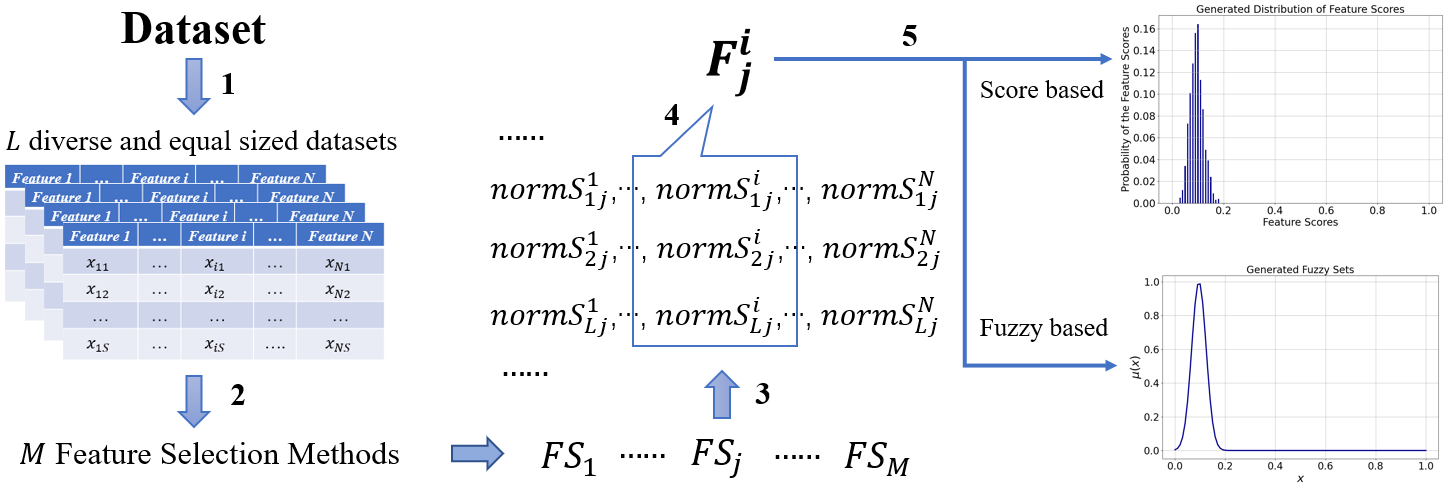
\includegraphics[width=1.75\columnwidth]{Figures/Step1_long.png}
	\caption{Process of the distribution generation of feature importance.}
	\label{step1}
\end{figure*}

\section{Methodology}
A similar ensemble framework is adopted from our previous research~\cite{shen2019novel}. Three main steps are followed in the framework, including: (1) distribution generation of feature importance; (2) distribution ensemble using fuzzy aggregation; (3) defuzzification for feature ranking. A score based distribution generation and weighted combination methods were used in our previous research~\cite{shen2019novel}. In contrast, alternative fuzzy-based distribution generation and aggregation method are proposed in this paper, as illustrated in Fig.~\ref{general_framework}.

\begin{figure}[h]
	\centering
	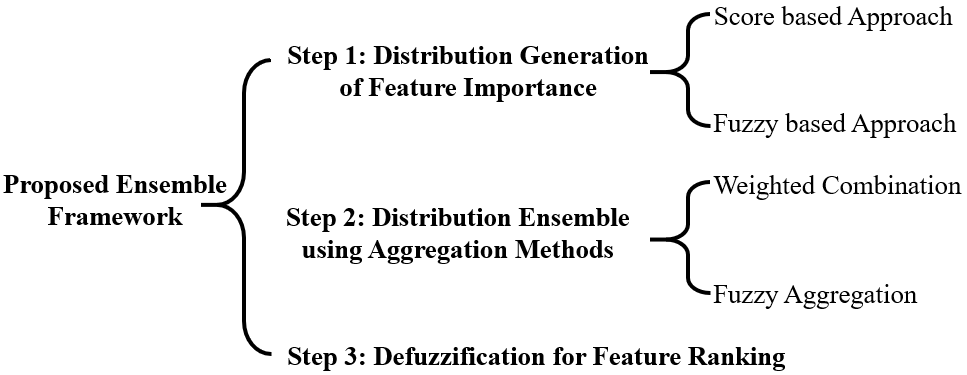
\includegraphics[width=1\columnwidth]{Figures/General_Framework.png}
	\caption{Overview of the proposed ensemble framework.}
	\label{general_framework}
\end{figure}


\subsection{Distribution Generation of Feature Importance}~\label{Step1_section}
To increase the generalizability of FS methods, bootstrap aggregation process is firstly applied to construct a number (denoted as $L$) of data subsets with $N$ features. $M$ different FS methods (denoted as $FS_j, j \in [1, ..., M]$) are then applied on these subsets to generate the feature scores for each subset per method. Distributions are constructed using $L$ bootstrap subsets to represent the importance of each feature. An overview of the distribution generation of feature importance is illustrated in Fig.~\ref{step1}. Detailed procedures are shown below.

\begin{figure*}[tb]
	\centering
	\begin{minipage}[t]{0.3\linewidth}
		\centering
		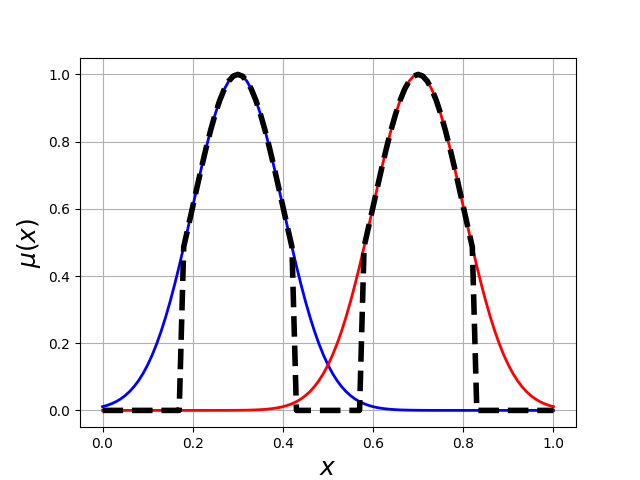
\includegraphics[width=1\textwidth]{Figures/Yager_class_w1000.png}
		\parbox{4cm}{\small \hspace{6.5cm}(a) Yager class with $\omega=1000$}
	\end{minipage}
	\hspace{1ex}
	\begin{minipage}[t]{0.3\linewidth}
		\centering
		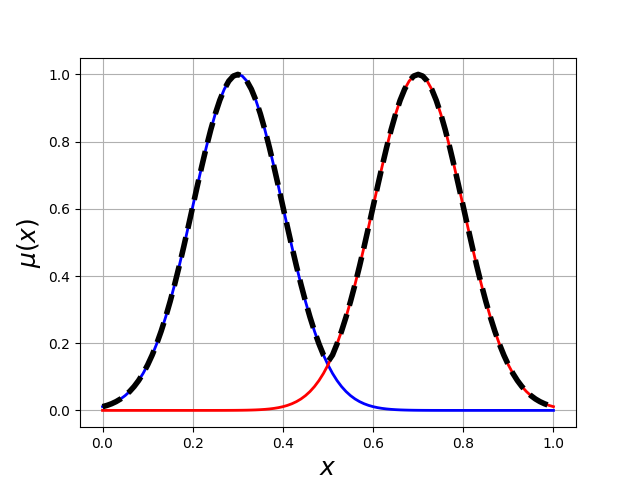
\includegraphics[width=1\textwidth]{Figures/Yager_class_w10.png}
		\parbox{4cm}{\small \hspace{5.5cm}(b) Yager class with $\omega=10$}
	\end{minipage}
	\hspace{1ex}
	\begin{minipage}[t]{0.3\linewidth}
		\centering
		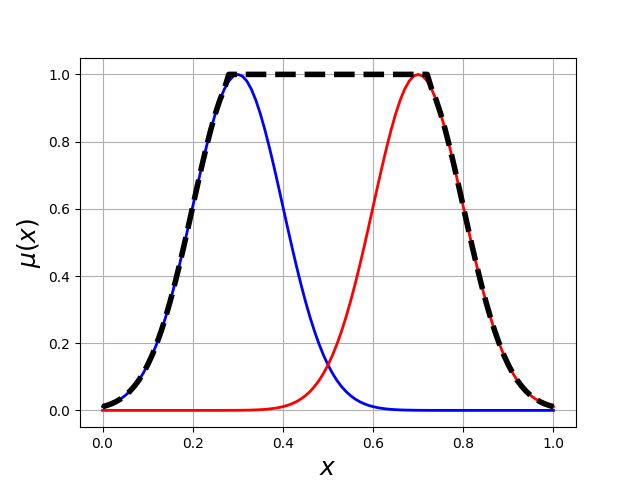
\includegraphics[width=1\textwidth]{Figures/Drastic_sum.png}
		\parbox{4cm}{\small \hspace{5.5cm}(b) Drastic sum}
	\end{minipage}
	\caption{Demonstration of fuzzy aggregation. Red and blue lines show the original fuzzy sets. Black dashed line indicates the fuzzy sets after aggregation.}
	\label{demon_fuzzy_agg}
\end{figure*}


\subsubsection{\textbf{Bootstrap Aggregation Process}}
Randomly select the samples and generate $L$ diverse and equal sized data subsets with replacement (denoted as $Subset l, (l \in [1, ..., L])$).

\subsubsection{\textbf{FS Method Deployment}}
Apply FS method $FS_j$ on $Subset \ l$ to get the feature score (denoted as $S^i_{j, l}$) of the $i$th feature ($i \in [1, ..., N]$). 

\subsubsection{\textbf{Feature Score Normalization}}
Normalize the feature scores of each FS method to the range of [0, 1] using min-max normalization~\cite{jain2005score} expressed in Equation~(\ref{min_max}).

\begin{equation}~\label{min_max}
	normS^i_{j, l} = \frac{S^i_{j, l} - min\{S_j\}}{max\{S_j\} - min\{S_j\}}
\end{equation}

\noindent
where $min\{S_j\}$ and $max\{S_j\}$ represent the min and max values of the feature scores generated by $FS_j$ for all features.


\subsubsection{\textbf{Feature Discretization}}
Each of the feature space is divided into 101 equal sized interval scores (set as $U$).

\begin{equation}
	U = \{0, 0.01, 0.02,..., 0.98, 0.99, 1\}
\end{equation}

Previously normalized feature scores are discretized and mapped into the corresponding element of set $U$ (denoted as $dS^i_{j, l}$), then combined into a list $F^i_j = \{ dS^i_{j, l} | l \in [1, ..., L]\}$.

\subsubsection{\textbf{Feature Importance Representation}}
Probability density function $PDF^i_j(x)$ (Equation (\ref{eq_pdf_score})) represents the feature scores which indicate the importance of the corresponding feature. The feature scores with higher PDF values are more representative for the features' importance. 

\begin{equation}~\label{eq_pdf_score}
	PDF^i_j(x)=\left\{
	\begin{array}{rcl}
		freq(x, F^i_j) / L      &      & {x \in   F^i_j}\\
		0     		&      & {x  \notin F^i_j}\\
	\end{array} \right.
\end{equation}

On account of the bootstrap process, the FS calculation of different subsets is regarded as independent and identically distributed (i.i.d) experiments. Based on Bernoulli's law of large numbers~\cite{grimmett2001probability}, for any positive number $\epsilon$, we have

\begin{equation}~\label{large_numbers}
	\lim \limits_{L \rightarrow \infty} P \{ |\frac{freq(x, F^i_j)}{L} - \mu| < \epsilon \} = 1
\end{equation}

Equation~(\ref{large_numbers}) indicates that when $L$ becomes large enough, $freq(x, F^i_j)/L$ can be used to represent the membership function values. The generation procedures are shown as below.

\begin{enumerate}
	\item Given FS method $FS_j$ and the $i$th feature, calculate the mean value $mean^i_j$, standard deviation $\delta^i_j$ and height $height^i_j$ from the probability density function $PDF^i_j(x)$.
	
	\item Constitute a normalized type-1 fuzzy set to represent the distribution of importance on the $i$th feature and $FS_j$, expressed in Equation~(\ref{fuzzy_sets}).
	
	\begin{equation}~\label{fuzzy_sets}
		Dist^i_j = \{  (x, \mu^i_j(x))  | x \in X  \}
	\end{equation}
	
	Based on Bernoulli's law of large numbers, distributions of membership functions are described as gaussian shaped. The membership function $\mu^i_j$ is constructed using Equation (\ref{gt_mu}).
	
	\begin{equation}~\label{gt_mu}
		\mu^i_j(x) = \frac{1}{\sqrt{2\pi}\delta^i_j}exp(- \frac{(x-mean^i_j)^2}{2(\delta^i_j)^2})
	\end{equation}	
\end{enumerate}



\subsection{Distribution Ensemble using Fuzzy Aggregation}
Fuzzy aggregation acts as the linear extensions of Boolean connectives within the scale between 0 and 1~\cite{mesiar2018aggregation}. In this paper, different fuzzy aggregation methods are implemented to combine the fuzzy sets generated in Section~\ref{Step1_section}. In the literature, various fuzzy aggregation operators are proposed, such as T-norm and S-norms. T-norm operators normally produce the intersection among fuzzy sets and eliminate other information outside the region, which lead to the loss of information during the aggregation process. On the other hand, S-norms are the generalized form of fuzzy union by integrating different fuzzy sets together, which retain most parts of information and are chosen in this research.

There are different kinds of S-norms, such as drastic sum, Dombi class, Yager class and etc. A parameterized family of S-norms Yager class is chosen on account that it covers different situations within the value range. Given $a$ and $b$ representing the membership function values of different fuzzy sets, Yager class is represented in Equation (\ref{yager_class}).

\begin{equation}~\label{yager_class}
	s_{\omega}(a, b) = min[1, (a^{\omega} + b^{\omega} )^{1/\omega}], \quad \omega \in (0, \infty)
\end{equation}

In the extreme case when $\omega$ becomes 0, Yager class turns to be drastic sum s-norm $s_{ds}(a, b)$.

\begin{equation}
	s_{ds}(a, b) = \left\{
	\begin{aligned}
		a  &  & if \ b  =  0 \\
		b  &  & if \ a=0 \\
		1  &  & otherwise
	\end{aligned}
	\right.
\end{equation}

The combined fuzzy sets after the aggregation process using Yager class with different parameters ($\omega=1000$, 10) and drastic sum S-norms are visualized in Fig.~\ref{demon_fuzzy_agg}.



\subsection{Defuzzification for Feature Ranking}
\subsubsection{\textbf{Defuzzification}}
After combining different fuzzy sets, a single value is computed using defuzzification processes. Centroid defuzzifier, or also called center of gravity defuzzifier is applied in the process~\cite{wang1996course}.

\subsubsection{\textbf{Feature Ranking}}
The feature ranking sequence is obtained from the highest to lowest values using the final defuzzified feature scores. Afterwards, the ranking sequence is utilized as the guidance for the subsequent decision making process.

\section{Method Evaluation}
In this section, datasets, experimental design, evaluation metrics and evaluation results are described.

\subsection{Datasets}
\subsubsection{\textbf{Training Data Repository}}
Eight datasets from UCI machine learning repository~\cite{Dua:2019} with different levels of data sparsity are chosen to tune the parameters of the proposed method. General information is shown in Table~\ref{data_training}.

\begin{table}[h]
	\centering
	\caption{General Description of Training Data Repository}
	\begin{tabular}{c c c c c c}
		\toprule
		\textbf{ID}   & \textbf{Datasets}  & $\#C$   &   $\#F$           &   $\#S$       &   $ \#S / \#C / \#F$  \\
		\midrule
		1      & Banknote                  & 2                & 4                   & 1372          &    171.5  \\
		2      & Mammographic         & 2                & 5                   & 830           &     83      \\
		3      & PIMA               		& 2                & 8                   & 768           &     48      \\ 
		4      & Statlog Heart      	   & 2                & 13                  & 270          &      10.4   \\ 
		5     & Seeds                         & 3                & 7                    & 210         &      10      \\
		6     & Sports Articles           & 2                & 59                  & 1000        &       8.5    \\
		7   & Parkinsons            	   & 2                & 22                  & 195         &       4.4    \\
		8   & Spectfheart                 & 2                & 44                  & 267         &       3.03  \\ 
		\bottomrule
	\end{tabular}
	\label{data_training}
\end{table}

$\#C$, $\#F$ and $\#S$ represent the number of classes, features and samples respectively. In the following tables, the datasets are represented using the ID numbers in the first column accordingly. 

\subsubsection{\textbf{Testing Data Repository}}
Another 8 datasets with different data sparsity are chosen for independent evaluation, as shown in Table~\ref{data_testing}. Those datasets are used for final performance analysis and comparison.

\begin{table}[h]
	\centering
	\caption{General Description of Testing Data Repository}
	\begin{tabular}{c c c c c c}
		\toprule
		\textbf{ID}   & \textbf{Datasets}  & \textbf{$\#C$}     &   $\#F$           &   $\#S$       &   $ \#S / (\#C \times \#F)$  \\
		\midrule
		9      & Yeast                         & 10              & 8                    &  1484        &   18.55 \\
		10      & CMSC                       & 2                & 18                  &  540           &   15     \\
		11      & WDBC                	     & 2                & 30                  &  569          &    9.48 \\ 		
		12      & Appendicitis              & 2                & 7                    & 106           &   7.57    \\
		13      & BCC                          & 2                & 9                    &  116           &   6.44   \\
		14      & Glass      	                 & 6                 & 9                    & 214           &    4.0     \\ 
		15      & Breast Tissue             & 6                 & 9                     & 106          &    2.0     \\ 
		16   &  Musk                            & 2                &  166                    &  476      &  1.43  \\
		\bottomrule
	\end{tabular}
	\label{data_testing}
\end{table}


\subsection{Selection of FS Methods}
\subsubsection{\textbf{Base Selectors}}
In our experiments, four representative algorithms (achieved superior performance in the literature) are selected from different filter FS categories~\cite{li2018feature}, which are implemented as the base selectors. General description of the chosen base selectors is shown in Table~\ref{fs_base}.

\begin{table}[h]\footnotesize
	\centering
	\caption{General Description of Base Selectors}
	\resizebox{0.5\textwidth}{!}{
	\begin{tabular}{c c c c c}
		\toprule
		\textbf{No.}   &  \textbf{Alias}    & \textbf{Name}   &   \textbf{Category}   \\
		\midrule
		1     &  CFS    &  Correlation based FS~\cite{hall1999correlation}      &  Statistical-based FS   \\
		2     &  ReliefF  &  ReliefF FS~\cite{robnik2003theoretical}     &   Similarity-based FS  \\
		3     &  MIFS     &  Mutual Information based FS~\cite{zaffalon2002robust}  & Information-based FS  \\
		4     &  IFS           &   Infinite based FS~\cite{roffo2015infinite}  & Graph-based FS  \\
		\bottomrule
	\end{tabular}
	}
	\label{fs_base}
\end{table}

\subsubsection{\textbf{The Proposed Ensemble Methods}}
Through incorporating different aggregation techniques, S-norms in Yager class (denoted as $F\_{Snorm}$) and the drastic sum fuzzy aggregation method (denoted as $F\_{DS}$) are used in our experiments. The performance of the proposed fuzzy based approaches are also compared with the score based method (denoted as $S\_{OW}$). $S\_{OW}$ method utilized the score based approach to generate the distributions and One Minus Standard Deviation Weights (OW) method for weighted combination, which is the best method reported in our previous research~\cite{shen2019novel}.

\subsection{Evaluation Metrics}~\label{eval_metrics}
Two metrics are used to evaluate the performance of FS methods on the aspects of accuracy and stability.

\subsubsection{\textbf{Evaluation on Accuracy}}~\label{eval_acc}
FS methods are ultimately used to improve the down-stream decision making performance (e.g. classification accuracy in our experiments) with simpler model and reduced number of features. After the pre-processing process using FS methods, the feature ranking sequence is obtained from the most to the least significant. Through gradually eliminating the unimportant features, predictive performance of FS methods is measured when combining with different decision making techniques. Detailed procedures are shown below.

\begin{enumerate}
	\item Divide the data into the training set and testing set using $K$-fold cross validation;
	\item Implement the given FS method on the training set to rank the features;
	\item Remove the least important feature one at a time. Use the retained features to train a model on the training set and make prediction on the testing set;
	\item For each reduced sized feature set, calculate the mean accuracy of all folds.
\end{enumerate}

After implementing those procedures, the accuracies using reduced feature sets and different FS methods can be visualized, as the example shown in Fig.~\ref{demonstration_acc}.

\begin{figure}[tb]
	\centering
	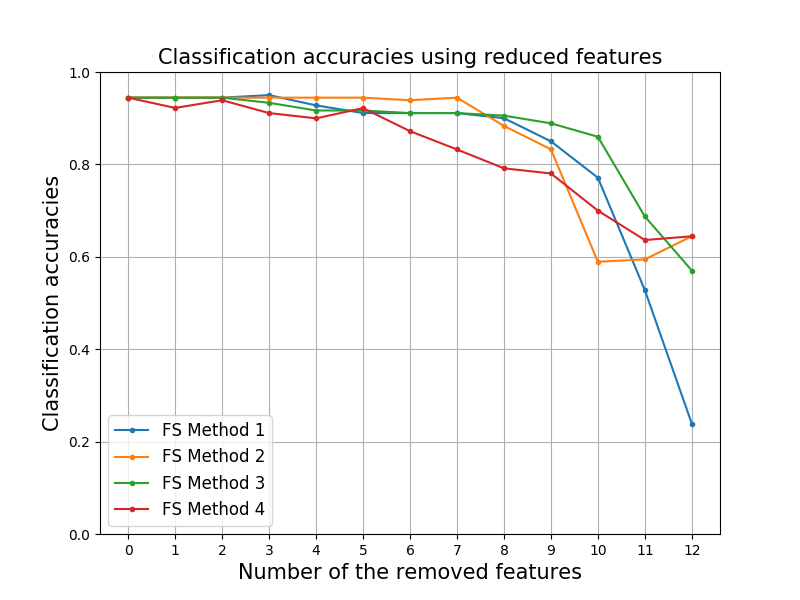
\includegraphics[width=0.5\textwidth]{Figures/classification_accuracy.png}
	\caption{Visualization of accuracies using removed features.}
	\label{demonstration_acc}
\end{figure}

For quantitative method comparison, a single value is normally summarized from these plots in Fig.~\ref{demonstration_acc}, such as mean, maximum or weighted sum~\cite{shen2020novel}. Here, we proposed a new evaluation metric in Equation (\ref{weighted_acc}), which is similar to the weighted sum~\cite{shen2020novel} in the calculation process and principle. However, this metric takes advantages of normalizing the performance score to the range of [0, 1], which is suitable for performance comparison among different datasets.

\begin{equation}\label{weighted_acc}
	Weighted \ Acc. =\frac{\sum Acc. * \% RemovedFeatures}{\sum \%RemovedFeatures}
\end{equation}

\noindent
where $\% RemovedFeatures$ represents the proportion of removed features. $Acc.$ indicates the classification accuracies based on the retained features. Based on Equation~(\ref{weighted_acc}), the accuracies using higher proportion of removed features have larger weights than others. 

\subsubsection{\textbf{Evaluation on Stability}}~\label{eval_sta}
To evaluate the stability of a given algorithm, recent research mainly focuses on the stability indices and introduces the metrics based on Hamming distance, correlation coefficients, consistency, information theory and etc~\cite{khaire2019stability}. A consistent feature ranking is more important than a fixed feature score in the context of FS. Hence rather than using Pearson's correlation to evaluate the feature score~\cite{shen2019novel}, Spearman's Rank Correlation Coefficient (SRCC) is implemented in this study to measure the difference between the ranking sequences generated from different folds in the cross-validation experiments.

\begin{equation}\label{stability}
	ASC = \frac{\sum_{x = 1}^{K} \sum_{y = x +1}^{K} SRCC(r^x, r^y)}{K(K-1)/2}
\end{equation}

\noindent
$SRCC(r_x, r_y)$ represents the SRCC between feature ranking sequences $r^x$ and $r^y$. $K$ stands for the number of folds. Equation (\ref{stability}) measures the average SRCC value for all pairwise comparisons of different folds.


\section{Experiments \& Results}
\subsection{Parameter Tuning using Training Data Repository}
In order to investigate the behavior of the proposed method when the parameter changes, the proposed method is firstly applied to the training data repository using 10-fold cross validation ($K=10$) for parameter tuning. Based on the sorted features, Random Forest is selected to model the classification process and calculate the accuracies on account of its bagging character and robustness to outliers and non-linear data. Performance of the FS methods is reported based on both accuracy and stability.

For the aims of tuning and selecting an optimal fuzzy aggregation approach, performance within the proposed ensemble FS framework using different fuzzy aggregation methods was compared. S-norms of Yager class with different parameters and drastic sum were utilized as the aggregation approaches. Within Yager class S-norms, the parameter $\omega$ was set as 1000, 10, 0.1 and 0.001 respectively. To compare the performance in the extreme case when $\omega = 0$, drastic sum is also applied as a supplementary.

\subsubsection{\textbf{Parameter Tuning on Accuracy}}
Based on Section~\ref{eval_acc}, comparison using accuracy evaluation metric is shown in Table~\ref{fuzzy_acc}.

\begin{table}[h]\scriptsize
	\centering
	\caption{Performance on Accuracy using Fuzzy based Approach}
		\begin{tabular}{c|c c c c |c}
			\toprule
			\multirow{2}{*}{\textbf{Data}}   & \multicolumn{4}{c|}{$F\_{Snorm}$ with different $\omega$}   & \multirow{2}{*}{$F\_{DS}$}  \\
		& 1000  & 10    & 0.1   & 0.001   &    \\ 
		\midrule
		1                              & \textbf{.864} (1.5) & .666 (4) & .673 (3) & \textbf{.864}  (1.5)   & \textbf{.864}   \\ 
		2                              & .769 (3) & .746 (4) & .772 (2) & \textbf{.827 (1)}   & \textbf{.827 }  \\ 
		3                              & .717 (3) & .706 (4) & \textbf{.744} (1) & .728  (2)       & .728   \\ 
		4                              & .705 (4) & .743 (1) & \textbf{.757} (1) & .730 (3)         & .730          \\ 
		5                              & .776 (3) & .756 (4) & .786 (2) & \textbf{.798}  (1)      & \textbf{.798}         \\ 
		6                              & .735 (4) & \textbf{.767} (1.5) & \textbf{.767} (1.5) & .761  (3)       & .761      \\ 
		7                              & .790 (3) & \textbf{.811} (1) & .793 (4) & .798 (2)        & .798    \\ 
		8                              & \textbf{.791} (1.5) & .788 (3) & .785 (4) & \textbf{.791} (1.5)      & \textbf{.791}   \\ 
		\midrule
		AVG                       & .768 (2.9) & .748 (2.8) & .760 (2.3) & .787 (1.9)      & .787   \\
		\bottomrule
	\end{tabular}
	\label{fuzzy_acc}
\end{table}

In Table~\ref{fuzzy_acc}, numbers in bold indicate the best performance for the given dataset. AVG means the average performance value among all the datasets in the table. The numbers in brackets represent the ranking index for $F\_{Snorm}$ using different parameters. Lower value indicates a higher rank and a better FS performance. In the case that more than one method obtained the same results, joint ranks were scored using the average value of the rank orders. For instance, ranking index 1 stands for the FS method achieved the best performance. When two methods achieved the same best performance, both of them were then scored 1.5.

It is seen from Table~\ref{fuzzy_acc} that $F\_{Snorm}$ achieved better performance with smaller parameter value $\omega$. When $\omega$ became close to 0 ($\omega = 0.001$ in this experiment), $F\_{Snorm}$ obtained the same optimal result as the drastic sum method $F\_{DS}$.


\subsubsection{\textbf{Parameter Tuning on Stability}}
Based on Section~\ref{eval_sta}, comparison using stability evaluation metric is shown in Table~\ref{fuzzy_sta}.

\begin{table}[h]\scriptsize
	\centering
	\caption{Performance on Stability using Fuzzy based Approach}
		\begin{tabular}{c|c c c c|c}
			\toprule
			\multirow{2}{*}{\textbf{Data}}  & \multicolumn{4}{c|}{$F\_{Snorm}$ with different $\omega$}    & \multirow{2}{*}{$F\_{DS}$}  \\
			& 1000         & 10          & 0.1            & 0.001          &   \\ 
			\midrule
			{1}     & \textbf{1.00} (2) & .960 (4) & \textbf{1.00} (2)  & \textbf{1.00} (2) & \textbf{1.00}   \\ 
			{2}     & .467 (4)    & .958  (2)     & .924  (3)         & \textbf{1.00} (1) & \textbf{1.00} \\ 
			{3}     & .733 (4)    & .961  (3)      & \textbf{1.00}  (1.5)        & \textbf{1.00} (1.5) & \textbf{1.00}  \\ 
			{4}     & .811  (4)   & .842   (3)        & .969    (2)       & \textbf{1.00} (1) & \textbf{1.00}  \\ 
			{5}     & .810  (4)   & .914   (2)   & .841  (3)            & \textbf{1.00} (1) & \textbf{1.00} \\ 
			{6}    & .513 (4)   & .869  (3)      & \textbf{.985} (1)            & .943  (2)        & .943             \\ 
			{7}    & .696  (4)      & .738    (3)      & .808    (2)     & \textbf{1.00} (1) & \textbf{1.00}  \\ 
			{8}    & \textbf{1.00}  (1.5)      & .784   (4)    & .932   (3)       & \textbf{1.00} (1.5) & \textbf{1.00}  \\ 
			\midrule
			{AVG}     & .754 (3.4)  & .878 (3)  & .932 (2.2) & \textbf{.993} (1.4)   & \textbf{.993}   \\
			\bottomrule
		\end{tabular}
	\label{fuzzy_sta}
\end{table}

In Table~\ref{fuzzy_sta}, the stability performance of $F\_{Snorm}$ method increased significantly with the decrease of parameter $\omega$ values in Yager class S-norms. When $\omega = 0.001$, $F\_{Snorm}$ achieved the best performance in 7 out of 8 datasets, which is the same as the drastic sum method $F\_{DS}$.

In summary, the fuzzy based approach using $F\_{Snorm}$ with $\omega$ close to 0 or the drastic sum method $F\_{DS}$ achieved the best performance on both accuracy and stability. As drastic sum is a simpler expression comparing with Yager class S-norms, $F\_{DS}$ is then chosen for further performance analysis and comparison using the test datasets.

\subsection{Performance Analysis using Testing Data Repository}
In this section, the performance of the fuzzy based approach is evaluated and analyzed on the testing data repository. To evaluate the effects of bootstrap aggregation process on FS results, performance of the proposed method is compared with the base selectors which utilized the same bootstrap aggregation process. Base selectors after bootstrap aggregation represent the FS methods which utilize bootstrap aggregation to generate the feature distributions and then defuzzify without any combination or aggregation procedures. In addition, the performance of the proposed fuzzy based approach is also compared with the score based approach in~\cite{shen2019novel}. The approach using One Minus Standard Deviation Weights combination method ($S\_{OW}$) has achieved the best performance hence been chosen here.

\subsubsection{\textbf{Performance Analysis on Accuracy}}
Based on Section~\ref{eval_acc}, comparison on accuracy is shown in Table~\ref{test_acc}. In the columns of base selectors after bootstrap aggregation, the operators (+/-) indicate that the bootstrap aggregation process has increased (+), decrease (-) or same (no mark) performance compared to the base selectors without bootstrap. The numbers in the brackets indicate the joint ranking index using the proposed method $S\_{OW}$ (before the slash) or $F\_{DS}$ (after the slash) comparing with the four base selectors after bootstrap aggregation. AVG stands for the average performance value for all datasets in terms of accuracy and ranking index.

\begin{table}[tb]\scriptsize
	\centering
	\caption{Performance Analysis on Accuracy}
	\resizebox{0.5\textwidth}{!}{
	\begin{tabular}{c|c c c c|c c}
		\toprule
		\multirow{2}{*}{\textbf{Data}}     & \multicolumn{4}{c|}{\textbf{Base Selectors with Bootstrap Aggregation}}      & \multicolumn{2}{c}{\textbf{Proposed Methods}}  \\ 
		& CFS            & ReliefF        & MIFS           & IFS   & $S\_{OW}$            & $F\_{DS}$    \\ 
		\midrule
		9                               & $ .439 $  (1.5/1.5)   & $ .351 $ (5/5) & $ .439 $ (1.5/1.5) &  $ .409 $ (3/3)      & $ .399 $ (4/)     & $ .391 $ (/4)      \\ 
		10                             & $ .915 $ (3/3)  & $ .915 $ (3/3)  & $ .915 $ (3/3) & $ .915 $ (3/3)                     & $ .915 $ (3/)  & $ .915 $ (/3)     \\ 
		11                             & $ .920 $ (4.5/4.5)  & $.920^-$ (4.5/4.5)  & $ .926 $ (1.5/1) & $ .922 $ (3/3)       & $ .926 $ (1.5/)  & $ .925 $ (/2)        \\ 
		12                             & $ .823^- $ (2/3)   & $ .836^- $ (1/1)  & $ .819^+ $ (3/4) & $ .806^+ $ (5/5)       & $ .817 $ (4/)     &  $ .832 $  (/2)      \\ 
		13                             & $ .307 $ (5/5) & $ .467^- $ (2/3)  & $ .521^- $ (1/1)   & $.404^-$  (3/4)       & $ .319 $ (4/)     & $ .519 $  (/2)       \\ 
		14                             & $ .349 $ (2/3) & $ .256 $ (5/5)  & $ .383^+ $  (1/1)  & $ .305^- $  (4/4)       & $ .309 $ (3/)     & $ .364 $ (/2)      \\ 
		15                             & $ .267 $ (5/5) & $ .303^- $ (1/2)  & $ .270^+ $ (4/4) & $ .297^+ $  (3/3)     & $ .301 $ (2/)      & $ .340 $ (/1)      \\ 
		16                             & $ .453^- $ (4/4)    & $ .440^- $ (5/5)  & $ .481^- $ (2.5/3) & $ .485^- $ (1/2)     & $ .481 $ (2.5/)  & $ .528 $  (/1)   \\ 
		\midrule
		AVG       & $ .559^- $ (3.4/3.6) & $ .561^- $ (3.3/3.5)   & $ .594^+ $ (2.2/2.3) & $ .568 $ (3.1/3.4)     & $ .559 $ (3/) & $ .602 $  (/2.1)  \\
		\bottomrule
	\end{tabular}
	}
	\label{test_acc}
\end{table}




In Table~\ref{test_acc}, our proposed methods $F\_{DS}$ produced overall better performance than $S\_{OW}$ and the four base selectors. It is also observed that the bootstrap aggregation for individual base selector does not lead to a higher accuracy in most cases for different datasets and FS methods. This indicates the improved accuracy mainly results from the proposed fuzzy aggregation method rather than the bootstrap process.

\subsubsection{\textbf{Performance Analysis on Stability}}
Based on Section~\ref{eval_sta}, performance comparison on stability is shown in Table~\ref{test_sta}.

\begin{table}[h]\scriptsize
	\centering
	\caption{Performance Analysis on Stability}
	\resizebox{0.5\textwidth}{!}{
	\begin{tabular}{c |c c c c|c  c  c} 
		\toprule
		\multirow{2}{*}{\textbf{Data}}  & \multicolumn{4}{c|}{\textbf{Base Selectors with Bootstrap Aggregation}} & \multicolumn{2}{c}{\textbf{Proposed Methods}}  \\
		& CFS   & ReliefF & MIFS  & IFS   & $S\_{OW}$            & $F\_{DS}$  \\ 
		\midrule
		9           & $ 1.00 $ (2/2.5)  & $ .995 $ (4.5/5)  & $ 1.00^+ $ (2/2.5) & $ 1.00 $ (2/2.5)    & $ .995 $ (4.5/) & $ 1.00 $ (/2.5)         \\ 
		10        & $ 1.00 $ (1/1.5)   & $ .854^+ $ (3/4)  & $ .856^+ $ (2/3) &  -$.078^+ $ (5/5)         & $ .672 $  (4/)    & $ 1.00 $  (/1.5)        \\ 
		11        & $ .949^+ $ (5/5)   & $ 1.00^+ $ (1/1.5)   & $ .989^+ $ (3/4)  & $ .995^+ $ (2/3)         & $ .988 $  (4/)    &  $ 1.00 $  (/1.5)   \\ 
		12        & $ .967^+ $ (1/2)   & $ .919^+ $ (3/4)   & $.941^+$ (2/3) & $ .917^+ $ (4/5)          & $ .815 $  (5/)    & $ 1.00 $  (/1)      \\ 
		13        & $ .915^+$ (3/4)   & $ .965^+ $ (2/3)   & $ .756^+ $ (5/5)  & $ .993^+ $ (1/2)        & $ .905 $  (4/)    &  $ 1.00 $  (/1)      \\ 
		14        & $ .972^+ $ (4/4)   & $ .980^+ $ (1/2)   & $ .890^+ $ (5/5) & $ .975 $  (3/3)           & $ .976 $  (2/)    &  $ 1.00 $  (/1)       \\ 
		15        & $ .667 $ (5/5)   & $ .980^- $ (1/2)    & $ .957^+ $ (2/3) & $ .944^+ $ (3/4)           & $ .922 $  (4/)    & $ 1.00 $  (/1)     \\ 
		16        & $ .935^+ $ (2/3)   & $ .887^+ $ (4/4)   & $ .886^+ $ (5/5) & $ .985 $ (1/2)           & $ .919 $  (3/)    &  $ 1.00 $  (/1)     \\ 
		\midrule
		Avg.     & $ .925^+ $ (2.9/3.4) & $ .948^+ $ (2.4/3.2)  & $ .909^+ $ (3.3/3.8) & $ .841^+ $ (2.6/3.3)     & $ .899 $ (3.8/)  &  $ 1.00 $  (/1.3)     \\
		\bottomrule
	\end{tabular}
	}
	\label{test_sta}
\end{table}

Comparing the performance of base selectors before and after bootstrap aggregation, the bagging process leads to increased stability in all the datasets. However, our proposed fuzzy based approach $F\_{DS}$ further outperformed the base selectors with bootstrap aggregation and $S\_{OW}$ in all datasets for stability measure. 

In summary, the proposed fuzzy based approach is able to achieve the overall best classification accuracy and the highest stability compared to the base selectors, which also outperformed our previously proposed score based method~\cite{shen2019novel}.


\section{Discussion \& Conclusion}
In this paper, an ensemble FS framework using fuzzy aggregation method has been proposed. By generating various distributions using the bootstrap approach, normalized fuzzy sets are utilized to represent the features' importance. Fuzzy aggregation approaches S-norms such as Yager class and drastic sum are implemented to aggregate the distributions from different FS methods. Through combining four state-of-the-art filter FS methods from different categories, our method produces a final score for feature ranking.

The proposed method was firstly evaluated on a training data repository for the purpose of parameter tuning for the proposed fuzzy aggregation method. It was subsequently evaluated on an independent testing data repository for performance comparison in terms of classification accuracy and stability. Our proposed method with drastic sum s-norms fuzzy aggregation has produced the best average classification accuracy of all the testing datasets. Additionally, it has also achieved significantly higher stability in all testing datasets.

In future work, we will compare the proposed method to other state-of-the-art FS approaches, and use more evaluation metrics such as robustness when incomplete data and outliers are considered.


%\clearpage

% The fuzzy similarity measure based framework will also be compared with other machine learning methods. \hl{}


% \section*{Acknowledgment}

% The preferred spelling of the word ``acknowledgment'' in America is without 
% an ``e'' after the ``g''. Avoid the stilted expression ``one of us (R. B. 
% G.) thanks $\ldots$''. Instead, try ``R. B. G. thanks$\ldots$''. Put sponsor 
% acknowledgments in the unnumbered footnote on the first page.

% \section*{References}


\bibliographystyle{IEEEtran}
%\bibliographystyle{unsrt}
\bibliography{sample}

\end{document}
